\documentclass[english,man]{apa6}

\usepackage{amssymb,amsmath}
\usepackage{ifxetex,ifluatex}
\usepackage{fixltx2e} % provides \textsubscript
\ifnum 0\ifxetex 1\fi\ifluatex 1\fi=0 % if pdftex
  \usepackage[T1]{fontenc}
  \usepackage[utf8]{inputenc}
\else % if luatex or xelatex
  \ifxetex
    \usepackage{mathspec}
    \usepackage{xltxtra,xunicode}
  \else
    \usepackage{fontspec}
  \fi
  \defaultfontfeatures{Mapping=tex-text,Scale=MatchLowercase}
  \newcommand{\euro}{€}
\fi
% use upquote if available, for straight quotes in verbatim environments
\IfFileExists{upquote.sty}{\usepackage{upquote}}{}
% use microtype if available
\IfFileExists{microtype.sty}{\usepackage{microtype}}{}

% Table formatting
\usepackage{longtable, booktabs}
\usepackage{lscape}
% \usepackage[counterclockwise]{rotating}   % Landscape page setup for large tables
\usepackage{multirow}		% Table styling
\usepackage{tabularx}		% Control Column width
\usepackage[flushleft]{threeparttable}	% Allows for three part tables with a specified notes section
\usepackage{threeparttablex}            % Lets threeparttable work with longtable

% Create new environments so endfloat can handle them
% \newenvironment{ltable}
%   {\begin{landscape}\begin{center}\begin{threeparttable}}
%   {\end{threeparttable}\end{center}\end{landscape}}

\newenvironment{lltable}
  {\begin{landscape}\begin{center}\begin{ThreePartTable}}
  {\end{ThreePartTable}\end{center}\end{landscape}}

  \usepackage{ifthen} % Only add declarations when endfloat package is loaded
  \ifthenelse{\equal{\string man}{\string man}}{%
   \DeclareDelayedFloatFlavor{ThreePartTable}{table} % Make endfloat play with longtable
   % \DeclareDelayedFloatFlavor{ltable}{table} % Make endfloat play with lscape
   \DeclareDelayedFloatFlavor{lltable}{table} % Make endfloat play with lscape & longtable
  }{}%



% The following enables adjusting longtable caption width to table width
% Solution found at http://golatex.de/longtable-mit-caption-so-breit-wie-die-tabelle-t15767.html
\makeatletter
\newcommand\LastLTentrywidth{1em}
\newlength\longtablewidth
\setlength{\longtablewidth}{1in}
\newcommand\getlongtablewidth{%
 \begingroup
  \ifcsname LT@\roman{LT@tables}\endcsname
  \global\longtablewidth=0pt
  \renewcommand\LT@entry[2]{\global\advance\longtablewidth by ##2\relax\gdef\LastLTentrywidth{##2}}%
  \@nameuse{LT@\roman{LT@tables}}%
  \fi
\endgroup}


  \usepackage{graphicx}
  \makeatletter
  \def\maxwidth{\ifdim\Gin@nat@width>\linewidth\linewidth\else\Gin@nat@width\fi}
  \def\maxheight{\ifdim\Gin@nat@height>\textheight\textheight\else\Gin@nat@height\fi}
  \makeatother
  % Scale images if necessary, so that they will not overflow the page
  % margins by default, and it is still possible to overwrite the defaults
  % using explicit options in \includegraphics[width, height, ...]{}
  \setkeys{Gin}{width=\maxwidth,height=\maxheight,keepaspectratio}
\ifxetex
  \usepackage[setpagesize=false, % page size defined by xetex
              unicode=false, % unicode breaks when used with xetex
              xetex]{hyperref}
\else
  \usepackage[unicode=true]{hyperref}
\fi
\hypersetup{breaklinks=true,
            pdfauthor={},
            pdftitle={Investigating the Interaction between Associative, Semantic, and Thematic Database Norms for Memory Judgments and Retrieval},
            colorlinks=true,
            citecolor=blue,
            urlcolor=blue,
            linkcolor=black,
            pdfborder={0 0 0}}
\urlstyle{same}  % don't use monospace font for urls

\setlength{\parindent}{0pt}
%\setlength{\parskip}{0pt plus 0pt minus 0pt}

\setlength{\emergencystretch}{3em}  % prevent overfull lines

\ifxetex
  \usepackage{polyglossia}
  \setmainlanguage{}
\else
  \usepackage[english]{babel}
\fi

% Manuscript styling
\captionsetup{font=singlespacing,justification=justified}
\usepackage{csquotes}
\usepackage{upgreek}

 % Line numbering
  \usepackage{lineno}
  \linenumbers


\usepackage{tikz} % Variable definition to generate author note

% fix for \tightlist problem in pandoc 1.14
\providecommand{\tightlist}{%
  \setlength{\itemsep}{0pt}\setlength{\parskip}{0pt}}

% Essential manuscript parts
  \title{Investigating the Interaction between Associative, Semantic, and
Thematic Database Norms for Memory Judgments and Retrieval}

  \shorttitle{Judgments and Recall}


  \author{Nicholas P. Maxwell\textsuperscript{1}~\& Erin M. Buchanan\textsuperscript{1}}

  % \def\affdep{{"", ""}}%
  % \def\affcity{{"", ""}}%

  \affiliation{
    \vspace{0.5cm}
          \textsuperscript{1} Missouri State University  }

  \authornote{
    Nicholas P. Maxwell is a graduate student at Missouri State University.
    Erin M. Buchanan is an Associate Professor of Psychology at Missouri
    State University.
    
    Correspondence concerning this article should be addressed to Nicholas
    P. Maxwell, 901 S. National Ave, Springfield, MO, 65897. E-mail:
    \href{mailto:maxwell270@live.missouristate.edu}{\nolinkurl{maxwell270@live.missouristate.edu}}
  }


  \abstract{This study examined the interactive relationship between semantic,
thematic, and associative word pair strength in the prediction of item
judgments and cued-recall performance. Participants were recruited from
Amazon's Mechanical Turk and were given word pairs of varying
relatedness to judge for their semantic, thematic, and associative
strength. After completing a distractor task, participants then
completed a cued recall task. First, we sought to expand previous work
on memory judgments to include three types of judgments of memory, while
also replicating bias and sensitivity findings. Next, we tested for an
interaction between the three database norms (FSG, COS, and LSA) when
predicting participant judgments and also extended previous work to test
for interactions between the three database norms when predicting
recall. Significant three-way interactions were found between FSG, COS,
and LSA when predicting judgments and recall. For low semantic feature
overlap, thematic and associative strength were competitive; as thematic
strength increased, associative predictiveness decreased. However, this
trend reversed for high semantic feature overlap, wherein thematic and
associative strength were complementary as both set of simple slopes
increased together. Overall, our findings indicate the degree to which
the processing of associative, semantic, and thematic information
impacts cognitive processes such as retrieval and item judgments, while
also examining the underlying, interactive relationship that exists
between these three types of information.}
  \keywords{judgments, memory, association, semantics, thematics \\

    
  }





\usepackage{amsthm}
\newtheorem{theorem}{Theorem}
\newtheorem{lemma}{Lemma}
\theoremstyle{definition}
\newtheorem{definition}{Definition}
\newtheorem{corollary}{Corollary}
\newtheorem{proposition}{Proposition}
\theoremstyle{definition}
\newtheorem{example}{Example}
\theoremstyle{definition}
\newtheorem{exercise}{Exercise}
\theoremstyle{remark}
\newtheorem*{remark}{Remark}
\newtheorem*{solution}{Solution}
\begin{document}

\maketitle

\setcounter{secnumdepth}{0}



The study of cognition has a rich history of exploring the role of
association in human memory. One key finding is that elements of
cognitive processing play a critical role in how well an individual
retains learned information. Throughout the mid-20th century,
researchers investigated this notion, particularly through the use of
paired-associate learning (PAL). In this paradigm, participants are
presented with a pair of items and are asked to make connections between
them so that the presentation of one item (the cue) will in turn trigger
the recall of the other (the target). Early studies of this nature
focused primarily on the effects of meaning and imagery on recall
performance. For example, Smythe and Paivio (1968) found that noun
imagery played a crucial role in PAL performance; subjects were much
more likely to remember word-pairs that were low in meaning similarity
if imagery between the two was high. Subsequent studies in this area
focused on the effects of mediating variables on PAL tasks as well as
the effects of imagery and meaningfulness on associative learning
(Richardson, 1998), with modern studies shifting their focus towards a
broad range of applied topics such as how PAL is affected by aging
(Hertzog, Kidder, Powell-Moman, \& Dunlosky, 2002), its impacts on
second language acquisition (Chow, 2014), and even in evolutionary
psychology (Schwartz \& Brothers, 2013).

Early PAL studies routinely relied on stimuli generated from word lists
that focused extensively on measures of word frequency, concreteness,
meaningfulness, and imagery (Paivio, 1969). However, the word pairs in
these lists were typically created due to their apparent relatedness or
frequency of occurrence in text. While lab self-generation appears face
valid, one finds that this method of selection lacks a decisive method
of defining the underlying relationships between the pairs (Buchanan,
2010), as these variables only capture psycholinguistic measurements of
an individual concept (i.e., how concrete is \emph{cat} and word
occurrence). PAL is, by definition, used on word pairs, which requires
examining concept relations in a reliable manner. As a result, free
association norms have become a common means of indexing associative
strength between word pairs (Nelson, McEvoy, \& Schreiber, 2004).

As we will use several related variables, it is important to first
define association as the context based relation between concepts,
usually found in text or popular culture (Nelson, McEvoy, \& Dennis,
2000). Such word associations typically arise through their
co-occurrence together in language. For example, the terms \emph{peanut}
and \emph{butter} have become associated over time through their joint
use to depict a particular type of food, though separately, the two
concepts share very little in terms of meaning. To generate these norms,
participants engage in a free association task, in which they are
presented with a cue word and are asked to list the first related target
word that comes to mind. The probability of producing a given response
to a particular cue word, or forward strength, can then be determined by
dividing the number of participants who produced the response in
question by the total number of responses generated for that word (FSG;
Nelson et al., 2000). Using this technique, researchers have developed
databases of associative word norms that can be used to generate stimuli
with a high degree of reliability. Many of these databases are now
readily available online, with the largest one consisting of over 72,000
associates generated from more than 5,000 cue words (Nelson et al.,
2004).

Similar to association norms, semantic word norms provide researchers
with another option of constructing stimuli for use in word-pair tasks.
These norms measure the underlying concepts represented by words and
allow researchers to tap into aspects of semantic memory. Semantic
memory is best described as an organized collection of our general
knowledge and contains information regarding a concept's meaning
(Hutchison, 2003). Models of semantic memory broadly fall into one of
two categories. Connectionist models (Rogers \& McClelland, 2006; e.g,
Rumelhart, McClelland, \& Group, 1986) portray semantic memory as a
system of interconnected units representing concepts, which are linked
together by weighted connections representing knowledge. By triggering
the input units, activation will then spread throughout the system
activating or suppressing connected units based on the weighted strength
of the corresponding unit connections (Jones, Willits, \& Dennis, 2015).
On the other hand, distributional models of semantic memory posit that
semantic representations are created through the co-occurrences of words
together in a body of text and suggest that words with similar meanings
will appear together in similar contexts (Riordan \& Jones, 2011).
Popular distributional models of semantic memory include Latent Semantic
Analysis (LSA; Landauer \& Dumais, 1997) and the Hyperspace Analogue to
Language (HAL; Lund \& Burgess, 1996).

Feature production tasks are a common means of producing semantic word
norms (Buchanan, Holmes, Teasley, \& Hutchison, 2013; McRae, Cree,
Seidenberg, \& McNorgan, 2005; Vinson \& Vigliocco, 2008) In such tasks,
participants are shown the name of a concept and are asked to list what
they believe the concept's most important features to be (McRae et al.,
2005). Several statistical measures have been developed which measure
the degree of feature overlap between concepts. Similarity between any
two concepts can be measured by representing them as vectors and
calculating the cosine value (COS) between them (Maki, McKinley, \&
Thompson, 2004). Cosine values range from 0 (unrelated) to 1 (perfectly
related). For example, the pair \emph{hornet} - \emph{wasp} has a COS of
.88, indicating a high degree of overlap between the two concepts.
Feature overlap can also be measured by JCN, which involves calculating
the information content value of each concept and the lowest
super-ordinate shared by each concept using an online dictionary, such
as WordNET (Miller, 1995). The JCN value is then computed by summing
together the difference of each concept and its lowest super-ordinate
(Jiang \& Conrath, 1997; Maki et al., 2004). The advantage to using COS
values over JCN values is the limitation of JCN being tied to a somewhat
static dictionary database, while a semantic feature production task can
be used on any concept to calculate COS values. However, JCN values are
less time consuming to obtain if both concepts are in the database
(Buchanan et al., 2013).

Semantic relations can be broadly described as being taxonomic or
thematic in nature. Whereas taxonomic relationships focus on the
connections between features and concepts within categories (e.g.,
\emph{bird} - \emph{pidgeon}), thematic relationships center around the
links between concepts and an overarching theme or scenario (e.g.,
\emph{bird} - \emph{nest}; Jones \& Golonka, 2012). Jouravlev and McRae
(2016) provide a list of 100 thematic relatedness production norms,
which were generated through a task similar to feature production in
which participants were presented with a concept and were asked to list
names of other concepts they believed to be related. Distributional
models of semantic memory also lend themselves well to the study of
thematic word relations. Because these models are text based and score
word pair relations in regard to their overall context within a
document, they assess thematic knowledge as well as semantic knowledge.
Additionally, text based models such as LSA are able to account for both
the effects of context and similarity of meaning, bridging the gap
between associations and semantics (Landauer, Foltz, \& Laham, 1998).

Discussion of these measures then leads to the question of whether each
one truly assesses some unique concept or if they simply tap into our
overall linguistic knowledge. Taken at face value, word pair
associations and semantic word relations appear to be vastly different,
yet the line between semantics/associations and thematics is much more
blurred. While thematic word relations are indeed an aspect of semantic
memory and include word co-occurrence as an integral part of their
creation, themes also appear to be indicative of a separate area of
linguistic processing. Previous research by Maki and Buchanan (2008)
appears to confirm this theory. Using clustering and factor analysis
techniques, they analyzed multiple associative, semantic, and text based
measures of associative and semantic knowledge. First, their findings
suggested associative measures to be separate from semantic measures.
Additionally, semantic information derived from lexical measures (e.g.,
COS, JCN) was found to be separate from measures generated from analysis
of text corpora, suggesting that text based measures may be more
representative of thematic information.

While it is apparent that these word relation measures are assessing
different domains of our linguistic knowledge, care must be taken when
building experimental stimuli through the use of normed databases, as
many word pairs overlap on multiple types of measurements, and even the
first studies on semantic priming used association word norms for
stimuli creation (Lucas, 2000; Meyer \& Schvaneveldt, 1971; Meyer,
Schvaneveldt, \& Ruddy, 1975). This observation becomes strikingly
apparent when one desires the creation of word pairs related on only one
dimension. One particular difficulty faced by researchers comes when
attempting to separate association strength from feature overlap, as
highly associated items tend to be semantically related as well.
Additionally, a lack of association strength between two items may not
necessarily be indicative of a total lack of association, as traditional
norming tasks typically do not produce a large enough set of responses
to capture all available associations between items. Some items with
extremely weak associations may inevitably slip through the cracks
(Hutchison, 2003). As such, the present study seeks to provide further
insight by examining how different levels of associative overlap
(measured in FSG), semantic overlap (feature overlap measured with COS),
and thematic overlap (measured with LSA) affect cognitive tasks such as
short term item retrieval and item relatedness judgments. Instead of
focusing solely on one variable or trying to create stimuli that
represent only one form of relatedness, we included a range of each of
these variables to explore their potential interaction.

Specifically, this research was conceptualized within the framework of a
three-tiered view of the interconnections between these systems as it
relates to processing concept information. The three-tiered view is
inspired by models of reading and naming, particularly the triangle
models presented by Seidenberg and Mcclelland (1989) and Plaut,
McClelland, Seidenberg, and Patterson (1996). These models explored the
nature of reading as bidirectional relations between semantics,
orthography, and phonology. In this research, we examine if the
semantic, associative, and thematic systems are interactive for judgment
and recall processes, much like the proposed interactive nature of
phonology, orthographics, and semantics for reading and naming
processes. Potentially, association, semantic, and thematic facets of
word relation each provide unique component that can be judged and used
for memory, thus, suggesting three separate networks of independent
information. This view seems unlikely, in that research indicates that
there is often overlap in the information provided by each measure of
word-pair relatedness. Instead, dynamic attractor networks, as proposed
by Hopfield (1982) and McLeod, Shallice, and Plaut (2000) may represent
better represent the interplay between these representations of
concepts, as these models posit a similar feedback relationship between
concepts in a network. Using these models as a theoretical framework for
our study, we sought to understand how these three types of word-pair
information may interact when judgment and recall processes were applied
to concept networks.

\subsection{Application to Judgment
Studies}\label{application-to-judgment-studies}

Traditional judgment of learning tasks (JOL) can be viewed as an
application of the PAL paradigm; participants are given pairs of items
and are asked to judge how accurately they would be able to correctly
match the target with the cue on a recall task. Judgments are typically
made out of 100, with a participant response of 100 indicating full
confidence in recall ability. In their 2005 study, Koriat and Bjork
examined overconfidence in JOLs by manipulating associative relations
(FSG) between word-pairs and found that subjects were more likely to
overestimate recall for pairs with little or no associative relatedness.
Additionally, this study found that when accounting for associative
direction, subjects were more likely to overestimate recall for pairs
that were high in backwards strength but low in forward strength. To
account for this finding, the authors suggested that JOLs may rely more
heavily on overlap between cue and target with the direction of the
associative relationship being secondary. Take for example the pair
\emph{feather} - \emph{bird}, which has a FSG of .051 and a BSG of .359.
This item pair also has a cosine value of .272 (suggesting low to
moderate feature overlap) and an LSA score of .517 (suggesting moderate
thematic overlap). As such, some of the overconfidence in JOLs may be
attributed more than just item associations. Paired items may also be
connected by similar themes or share certain features, resulting in
inflated JOLs.

JOL tasks can then be manipulated to investigate perceptions of word
pair relationships by having participants judge how related they believe
the stimuli to be (Maki, 2007a, 2007b). The judged values generated from
this task can then be compared to the normed databases to create a
similar accuracy function or correlation as is created in JOL studies.
When presented with the item pair, participants are asked to estimate
the number of people out of 100 who would provide the target word when
shown only the cue (Maki, 2007b), which mimics how the association word
norms are created through free association tasks. Maki (2007a)
investigated such judgments within the context of associative memory by
having participants rate how much associative overlap was shared between
items and found that responses greatly overestimated the actual overlap
strength for pairs that were weak associates, while underestimating
strong associates; thus replicating the Koriat and Bjork (2005) findings
for judgments on associative memory, rather than on learning.

The judgment of associative memory function (JAM) is created by plotting
the judged values by the word pair's normed associative strength and
calculating a fit line, which characteristically has a high intercept
(bias) with a shallow slope (sensitivity). Figure \ref{fig:makislope}
illustrates this function. Overall, the JAM function has been found to
be highly reliable and generalized well across multiple variations of
the study, with item characteristics such as word frequency, cue set
size (QSS), and semantic similarity all having a minimal influence on it
(Maki, 2007b). Furthermore, an applied meta-analysis of more than ten
studies on JAM indicated that bias and sensitivity are nearly
unchangeable, often hovering around 40-60 points for the intercept and
.20-.30 for the slope (Valentine \& Buchanan, 2013). Additionally,
Valentine and Buchanan (2013) extended this research to include
judgments of semantic memory with the same results.

\begin{figure}
\centering
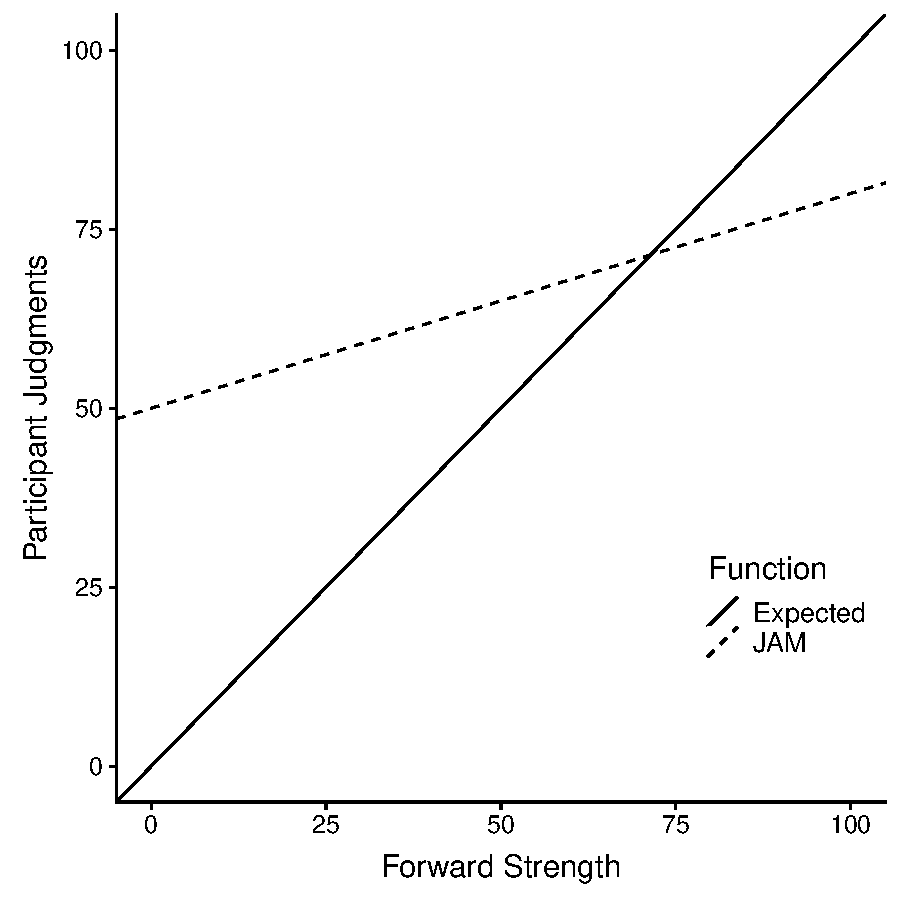
\includegraphics{max_buch_JOL_files/figure-latex/makislope-1.pdf}
\caption{\label{fig:makislope}JAM slope findings from Maki (2007a). JAM is
characterized by a high intercept (between 40 and 60) and a shallow
slope (between 0.20 and 0.40). The solid line shows expected results if
judgment ratings are perfectly calibrated with association norms.}
\end{figure}

The present study combined PAL and JAM to examine item recall within the
context of item judgments, while extending the Maki's JAM task to
include judgments of both semantic and thematic memory. Relationship
strengths between word pairs were manipulated across each of the three
types of memory investigated. Previous research on normed databases was
used to assure a range of item relatedness. We tested the following
hypotheses:

\begin{enumerate}
\def\labelenumi{\arabic{enumi})}
\item
  First, we sought to expand previous Maki (2007b), Maki (2007a),
  Buchanan (2010), and Valentine and Buchanan (2013) research to include
  three types of judgments of memory in one experiment, while
  replicating JAM bias and sensitivity findings. We used the three
  database norms for association, semantics, and thematics to predict
  each type of judgment and calculated average slope and intercept
  values for each participant. We expected to find slope and intercept
  values that were significantly different from zero, as well as within
  the range of previous findings. Additionally, we examined the
  frequency of each predictor being the strongest variable to predict
  its own judgment condition (i.e., how often association was the
  strongest predictor of associative judgments, etc.).
\item
  Given the overlap in these variables and predictions from
  bidirectional models, we expected to find an interaction between
  database norms in predicting participant judgments, controlling for
  judgment type. We used multilevel modeling to examine that interaction
  of database norms for association, semantics, and thematics in
  relation to participant judgments.
\item
  These analyses were then extended to recall as the dependent variable
  of interest. We examined the interaction of database norms in
  predicting recall by using a multilevel logistic regression, while
  controlling for judgment type and rating. We expected to find that
  database norms would show differences in recall based on the levels
  other variables (the interaction would be significant), and that
  ratings would also positively predict recall (i.e., words that
  participants thought were more related would be remembered better).
\item
  Finally, we examined if the judgment slopes from Hypothesis 1 would be
  predictive of recall. Hypothesis 3 examined the direct relationship of
  word relatedness on recall, while this hypothesis explored if
  participant sensitivity to word relatedness was a predictor of recall.
  For this analysis, we used a multilevel logistic regression to control
  for multiple judgment slope conditions.
\end{enumerate}

\section{Methods}\label{methods}

\subsection{Participants}\label{participants}

A power analysis was conducted using the \emph{simR} package in \emph{R}
(Green \& MacLeod, 2016). This package uses simulations to generate
power estimates for mixed linear models created from the \emph{lme4}
package in \emph{R} (Bates, Mächler, Bolker, \& Walker, 2015). The
results of this analyses suggested a minimum of 35 participants would be
required to detect an effect. However, because power often tends to be
underestimated, we extended participant recruitment as funding
permitted. In total, 112 participants took part in this study.
Participants were recruited from Amazon's Mechanical Turk, which is a
website that allows individuals to host projects and connects them with
a large pool of respondents who complete them for small amounts of money
(Buhrmester, Kwang, \& Gosling, 2011). Participant responses were
screened for a basic understanding of the study's instructions. Common
reasons for rejecting responses included participants entering related
words when numerical judgment responses were required, and participants
responding to the cue words during the recall phase with sentences or
phrases instead of individual words. Those that completed the study
correctly were compensated \$1.00 for their participation.

\subsection{Materials}\label{materials}

The stimuli used were sixty-three words pairs of varying associative,
semantic, and thematic relatedness which were created from the Buchanan
et al. (2013) word norm database and website. Associative relatedness
was measured with Forward Strength (FSG), which is the probability that
a cue word will elicit a desired target word (Nelson et al., 2004). This
variable ranges from zero to one wherein zero indicates no association,
while one indicates that participants would always give a target word in
response to the cue word. Semantic relatedness was measured with Cosine
(COS), which is a measure of semantic feature overlap (Buchanan et al.,
2013; McRae et al., 2005; Vinson \& Vigliocco, 2008). This variable
ranges from zero to one where zero indicates no shared semantic features
between concepts and higher numbers indicate more shared features
between concepts. Thematic relatedness was calculated with Latent
Semantic Analysis (LSA), which generates a score based upon the
co-occurrences of words within a document (Landauer \& Dumais, 1997;
Landauer et al., 1998). LSA values also range from zero to one,
indicates no co-occurrence at the low end and higher co-occurrence with
higher values. These values were chosen to represent these categories
based on face validity and previous research on how word pair
psycholinguistic variables overlap (Maki \& Buchanan, 2008).

Stimuli were varied such that each variable included a range of each
variable. See Table \ref{tab:stim-table} for stimuli averages, SD, and
ranges. A complete list of stimuli can be found at
\url{http://osf.io/y8h7v}. The stimuli were arranged into three blocks
for each judgment condition described below wherein each block contained
21 word pairs. Due to limitations of the available stimuli, blocks were
structured so that each one contained seven word pairs of low (0-.33),
medium (.34-.66), and high (.67-1.00) COS relatedness. Because of this
selection process, FSG and LSA strengths are contingent upon the
selected stimuli's COS strengths. We selected stimuli within the cosine
groupings to cover a range of FSG and LSA values, but certain
combinations are often difficult to achieve. For example, there are only
four word-pairs that are both high COS and high FSG, thus limiting the
ability to manipulate LSA. The study was built online using Qualtrics,
and three surveys were created to counter-balance the order in which
blocks appeared. Each word pair appeared counter-balanced across each
judgment condition, and stimuli were randomized within each block.

\begin{table}[tbp]
\begin{center}
\begin{threeparttable}
\caption{\label{tab:stim-table}Summary Statistics for Stimuli}
\begin{tabular}{lccccccccc}
\toprule
Variable &   & COS Low &   &   & COS Average &   &   & COS High &  \\
\midrule
 & $N$ & $M$ & $SD$ & $N$ & $M$ & $SD$ & $N$ & $M$ & $SD$\\
COS & 21 & .115 & .122 & 21 & .461 & .098 & 21 & .754 & .059\\
FSG Low & 18 & .062 & .059 & 18 & .122 & .079 & 17 & .065 & .067\\
FSG Average & 3 & .413 & .093 & 2 & .411 & .046 & 2 & .505 & .175\\
FSG High & NA & NA & NA & 1 & .697 & NA & 2 & .744 & .002\\
LSA Low & 16 & .174 & .090 & 8 & .220 & .074 & 7 & .282 & .064\\
LSA Average & 5 & .487 & .126 & 10 & .450 & .111 & 12 & .478 & .095\\
LSA High & NA & NA & NA & 3 & .707 & .023 & 2 & .830 & .102\\
\bottomrule
\addlinespace
\end{tabular}
\begin{tablenotes}[para]
\textit{Note.} COS: Cosine, FSG: Forward Strength, LSA: Latent Semantic Analysis.
\end{tablenotes}
\end{threeparttable}
\end{center}
\end{table}

\subsection{Procedure}\label{procedure}

The present study was divided into three phases. In the first section,
participants were presented with word pairs and were asked to make
judgments of how related they believed the words in each pair to be.
This judgment phase consisted of three blocks of 21 word pairs which
corresponded to one of three types of word pair relationships:
associative, semantic, or thematic. Each block was preceded by a set of
instructions explaining one of the three types of relationships, and
participants were provided with examples which illustrated the type of
relationship to be judged. Participants were then presented with the
word pairs to be judged. The associative block began by explaining
associative memory and the role of free association tasks. Participants
were provided with examples of both strong and weak associates. For
example, \emph{lost} and \emph{found} and were presented as an example
of a strongly associated pair, while \emph{article} was paired with
\emph{newspaper}, \emph{the}, and \emph{clothing} to illustrate that
words can have many weak associates. The semantic judgment block
provided participants with a brief overview of how words are related by
meaning and showed examples of concepts with both high and low feature
overlap. \emph{Tortoise} and \emph{turtle} were provided as an example
of two concepts with significant overlap. Other examples were then
provided to illustrate concepts with little or no overlap. For the
thematic judgments, participants were provided with an explanation of
thematic relatedness. \emph{Tree} is explained to be related to
\emph{leaf}, \emph{fruit}, and \emph{branch}, but not \emph{computer}.
Participants were then given three concepts (\emph{lost}, \emph{old},
\emph{article}) and were asked to come up with words that they feel are
thematically related.

After viewing the examples at the start of the block, participants
completed the judgment task. Judgment instructions for each block were
contingent upon the type of judgment being elicited. For example,
instructions in the associative block asked participants to estimate how
many college students out of 100 would respond to the cue word with
given target, while instructions for semantic judgments asked
participants to indicate the percent of features shared between two
concepts. The complete experiment can be found at
\url{http://osf.io/y8h7v}, which contains the exact instructions given
to participants for each block and displays the structure of the study.
All judgment instructions were modeled after Buchanan (2010) and
Valentine and Buchanan (2013).

Participants then rated the relatedness of the word pairs based on the
set of instructions that they received. In accordance with previous work
on JOLs and JAM, item judgments were made using a scale of zero to one
hundred, with zero indicating no relationship, and one hundred
indicating a perfect relationship. Participants typed their responses
into the survey. Once completed, participants then completed the
remaining judgment blocks in the same manner. Each subsequent judgment
block changed the type of judgment being made. Three versions of the
study were created, which counter-balanced the order in which the
judgment blocks appeared, and participants were randomly assigned to a
survey version. This resulted in each word pair receiving judgments on
each of the three types relationships. After completing this section,
participants were then presented with a short distractor task to account
for recency effects. In this section, participants were presented with a
randomized list of the fifty U.S. states and were asked to arrange them
in alphabetical order. This task was timed to last two minutes. Once
time had elapsed, participants automatically progressed to the final
section, which consisted of a cued-recall task. Participants were
presented with each of the 63 cue words from the judgment section and
were asked to complete each word pair by responding with the correct
target word. Participants were informed that they would not be penalized
for guessing. The cued-recall task included all stimuli in a random
order.

\section{Results}\label{results}

\subsection{Data Processing and Descriptive
Statistics}\label{data-processing-and-descriptive-statistics}

First, the recall portion of the study was coded as zero for incorrect
responses, one for correct responses, and NA for participants who did
not complete the recall section (all or nearly all responses were
blank). All word responses to judgment items were deleted and set to
missing data. The final dataset was created by splitting the initial
data file into six sections (one for each of the three experimental
blocks and their corresponding recall scores). Each section was
individually melted using the \emph{reshape} package in \emph{R}
(Wickham, 2007) and was written as a csv file. The six output files were
then combined to form the final dataset. Code is available on our OSF
page embedded inline with the manuscript in an \emph{R} markdown
document (Aust \& Barth, 2017). With 112 participants, the dataset in
long format included 7,056 rows of potential data (i.e., 112
participants * 63 judgments). One incorrect judgment data point
(\textgreater{} 100) was corrected to NA. Missing data for judgments or
recall were then excluded from the analysis, which includes word
responses to judgment items (i.e., responding with \emph{cat} instead of
a number). These items usually excluded a participant from receiving
Amazon Mechanical Turk payment, but were included in the datasets found
online. In total, 787 data points were excluded (188 judgment only, 279
recall only, 320 both), leading to a final \emph{N} of 105 participants
and 6,269 observations. Recall and judgment scores were then screened
for outliers using Mahalanobis distance at \emph{p} \textless{} .001,
and no outliers were found (Tabachnick \& Fidell, 2007). To screen for
multicollinearity, we examined correlations between judgment items, COS,
LSA, and FSG. All correlations were \emph{r}s \textless{} .50.

The mean judgment of memory for the associative condition (\emph{M} =
58.74, \emph{SD} = 30.28) was lower than the semantic (\emph{M} = 66.98,
\emph{SD} = 28.31) and thematic (\emph{M} = 71.96, \emph{SD} = 27.80)
judgment conditions. Recall averaged over 60\% for all three conditions:
associative \emph{M} = 63.40, \emph{SD} = 48.18; semantic \emph{M} =
68.02, \emph{SD} = 46.65; thematic \emph{M} = 64.89, \emph{SD} = 47.74.

\subsection{Hypothesis 1}\label{hypothesis-1}

\begin{table}[tbp]
\begin{center}
\begin{threeparttable}
\caption{\label{tab:hyp1-table1}Summary Statistics for Hypothesis 1 t-Tests}
\begin{tabular}{lccccccc}
\toprule
Variable & $M$ & $SD$ & $t$ & $df$ & $p$ & $d$ & $95\% CI$\\
\midrule
Associative Intercept & .511 & .245 & 20.864 & 99 & < .001 & 2.086 & 1.734 - 2.435\\
Associative COS & -.030 & .284 & -1.071 & 99 & .287 & -0.107 & -0.303 - 0.090\\
Associative FSG & .491 & .379 & 12.946 & 99 & < .001 & 1.295 & 1.027 - 1.559\\
Associative LSA & .035 & .317 & 1.109 & 99 & .270 & 0.111 & -0.086 - 0.307\\
Semantic Intercept & .587 & .188 & 31.530 & 101 & < .001 & 3.122 & 2.649 - 3.592\\
Semantic COS & .059 & .243 & 2.459 & 101 & .016 & 0.244 & 0.046 - 0.440\\
Semantic FSG & .118 & .382 & 3.128 & 101 & .002 & 0.310 & 0.110 - 0.508\\
Semantic LSA & .085 & .304 & 2.816 & 101 & .006 & 0.279 & 0.080 - 0.476\\
Thematic Intercept & .656 & .186 & 35.475 & 100 & < .001 & 3.530 & 3.002 - 4.048\\
Thematic COS & -.081 & .239 & -3.405 & 100 & < .001 & -0.339 & -0.539 - -0.137\\
Thematic FSG & .192 & .306 & 6.290 & 100 & < .001 & 0.626 & 0.411 - 0.838\\
Thematic LSA & .188 & .265 & 7.111 & 100 & < .001 & 0.708 & 0.488 - 0.924\\
\bottomrule
\addlinespace
\end{tabular}
\begin{tablenotes}[para]
\textit{Note.} Confidence interval for $d$ was calculated using the non-central $t$-distribution. 
\end{tablenotes}
\end{threeparttable}
\end{center}
\end{table}

Our first hypothesis sought to replicate bias and sensitivity findings
from previous research while expanding the JAM function to include
judgments based on three types of memory. FSG, COS, and LSA were used to
predict each type of judgment. Judgment values were divided by 100, so
as to place them on the same scale as the database norms. Slopes and
intercepts were then calculated for each participant's ratings for each
of the three judgment conditions, as long as they contained at least
nine data points out of the 21 that were possible. Single sample
\emph{t}-tests were then conducted to test if slope and intercept values
significantly differed from zero. See Table \ref{tab:hyp1-table1} for
means and standard deviations. Slopes were then compared to the JAM
function, which is characterized by high intercepts (between 40 and 60
on a 100 point scale) and shallow slopes (between 20 and 40). Because of
the scaling of our data, to replicate this function, we should expect to
find intercepts ranging from .40 to .60 and slopes in the range of 0.20.
to 0.40. Intercepts for associative, semantic, and thematic judgments
were each significant, and all fell within or near the expected range.
Thematic judgments had the highest intercept at .656, while associative
judgments had the lowest intercept at .511.

The JAM slope was successfully replicated for FSG in the associative
judgment condition, with FSG significantly predicting association,
although the slope was slightly higher than expected at .491. COS and
LSA did not significantly predict association. For semantic judgments,
each of the three database norms were significant predictors. However,
JAM slopes were not replicated for this judgment type, as FSG had the
highest slope at .118, followed by LSA .085, and then COS .059. These
findings were mirrored for thematic judgments, as each database norm was
a significant predictor, yet slopes for each predictor fell below range
of the expected JAM slopes. Again, FSG had the highest slope, this time
just out of range at .192, followed closely by LSA at .188.
Interestingly, COS slopes were found to be negative for this judgment
condition, -.081. Overall, although JAM slopes were not successfully
replicated in each judgment type, the high intercepts and shallow slopes
present in all three judgment conditions are still indicative of
overconfidence and insensitivity in participant judgments.

Additionally, we examined the frequency that each predictor was the
maximum strength for each judgment condition. For the associative
condition, FSG was the strongest predictor for 64.0 of the participants,
with COS and LSA being the strongest for only 16.0 and 20.0 of
participants respectively. These differences were less distinct when
examining the semantic and thematic judgment conditions. In the semantic
condition, FSG was highest at 44.1 of participants, LSA was second at
32.4, and COS was least likely at 23.5. Finally, in the thematic
condition, LSA was most likely to be the strongest predictor with 44.6
of participants, with FSG being the second most likely at 36.6, and COS
again being least likely at 18.8. Interestingly, in all three
conditions, COS was least likely to be the strongest predictor, even in
the semantic judgment condition.

\subsection{Hypothesis 2}\label{hypothesis-2}

\begin{table}[tbp]
\begin{center}
\begin{threeparttable}
\caption{\label{tab:hyp2-table}MLM Statistics for Hypothesis 2}
\small{
\begin{tabular}{lcccc}
\toprule
Variable & \multicolumn{1}{c}{$beta$} & \multicolumn{1}{c}{$SE$} & \multicolumn{1}{c}{$t$} & \multicolumn{1}{c}{$p$}\\
\midrule
Intercept & 0.603 & 0.014 & 43.287 & < .001\\
Semantic Judgments & 0.079 & 0.008 & 9.968 & < .001\\
Thematic Judgments & 0.127 & 0.008 & 16.184 & < .001\\
ZCOS & -0.103 & 0.017 & -6.081 & < .001\\
ZLSA & 0.090 & 0.022 & 4.196 & < .001\\
ZFSG & 0.271 & 0.029 & 9.420 & < .001\\
ZCOS:ZLSA & -0.141 & 0.085 & -1.650 & .099\\
ZCOS:ZFSG & -0.374 & 0.111 & -3.364 & < .001\\
ZLSA:ZFSG & -0.569 & 0.131 & -4.336 & < .001\\
ZCOS:ZLSA:ZFSG & 3.324 & 0.490 & 6.791 & < .001\\
Low COS ZLSA & 0.129 & 0.033 & 3.934 & < .001\\
Low COS ZFSG & 0.375 & 0.049 & 7.679 & < .001\\
Low COS ZLSA:ZFSG & -1.492 & 0.226 & -6.611 & < .001\\
High COS ZLSA & 0.051 & 0.031 & 1.647 & .100\\
High COS ZFSG & 0.167 & 0.034 & 4.878 & < .001\\
High COS ZLSA:ZFSG & 0.355 & 0.143 & 2.484 & .013\\
Low COS Low LSA ZFSG & 0.663 & 0.078 & 8.476 & < .001\\
Low COS High LSA ZFSG & 0.087 & 0.049 & 1.754 & .079\\
Avg COS Low LSA ZFSG & 0.381 & 0.047 & 8.099 & < .001\\
Avg COS High LSA ZFSG & 0.161 & 0.027 & 5.984 & < .001\\
High COS Low LSA ZFSG & 0.099 & 0.058 & 1.707 & .088\\
High COS High LSA ZFSG & 0.236 & 0.023 & 10.263 & < .001\\
\bottomrule
\addlinespace
\end{tabular}
}
\begin{tablenotes}[para]
\textit{Note.} Database norms were mean centered. The table shows main effects and interactions for database norms at low, average, and high levels of COS and LSA when predicting participant judgments.
\end{tablenotes}
\end{threeparttable}
\end{center}
\end{table}

\begin{figure}
\centering
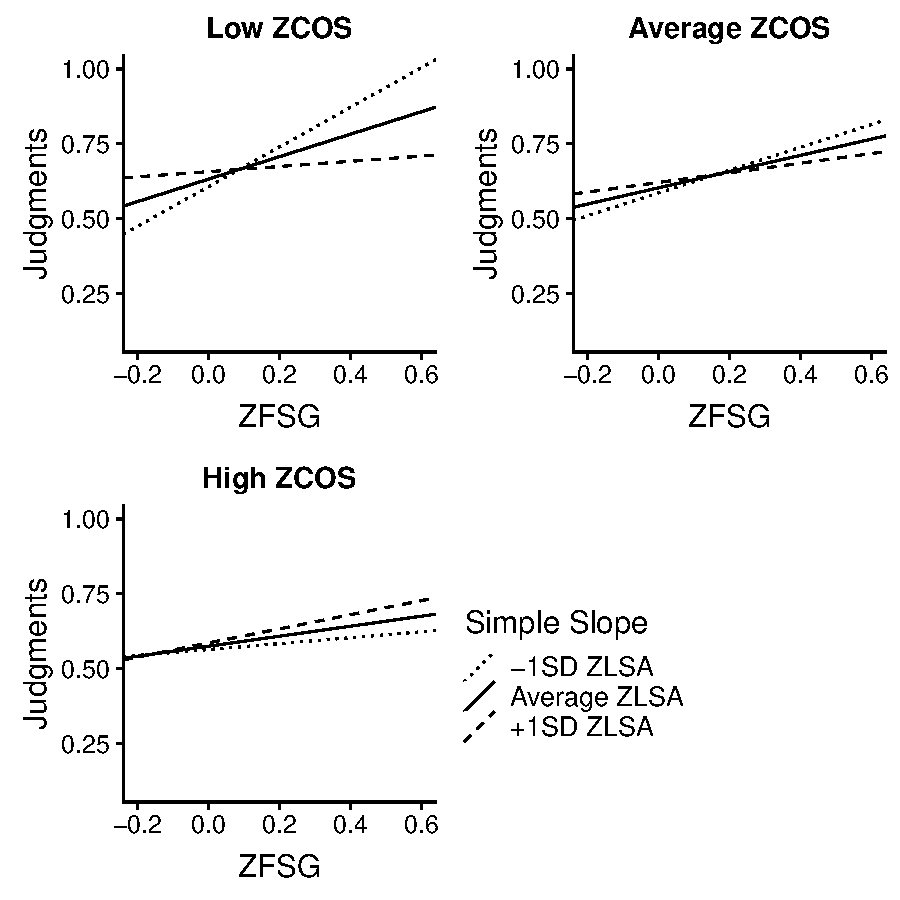
\includegraphics{max_buch_JOL_files/figure-latex/hyp2graph-1.pdf}
\caption{\label{fig:hyp2graph}Simple slopes graph displaying the slope of
FSG when predicting participant judgments at low, average, and high LSA
split by low, average, and high COS. All variables were mean centered.}
\end{figure}

As a result of the overlap between variables in Hypothesis 1, the goal
of Hypothesis 2 was to test for an interaction between the three
database norms when predicting participant judgment ratings. First, the
database norms were mean centered to control for multicollinearity. The
\emph{nlme} package and \emph{lme} function were used to calculate these
analyses (Pinheiro, Bates, Debroy, Sarkar, \& R Core Team, 2017). A
maximum likelihood multilevel model was used to test the interaction
between FSG, COS, and LSA when predicting judgment ratings while
controlling for type of judgment, with participant number being used as
the random intercept factor. Multilevel models were used to retain all
data points (rather than averaging over items and conditions), while
controlling for correlated error due to participants, as these models
are advantageous for multiway repeated measures designs (Gelman, 2006).
This analysis resulted in a significant three-way interaction between
FSG, COS, and LSA (\(\beta\) = 3.324, \emph{p} \textless{} .001), which
is examined below in a simple slopes analysis. Table
\ref{tab:hyp2-table} includes values for main effects, two-way, and
three-way interactions.

To investigate this interaction, simple slopes were calculated for low,
average, and high levels of COS. This variable was chosen for two
reasons: first, it was found to be the weakest of the three predictors
in hypothesis one, and second, manipulating COS would allow us to track
changes across FSG and LSA. Significant two-way interactions were found
between FSG and LSA at both low COS (\(\beta\) = -1.492, \emph{p}
\textless{} .001), average COS (\(\beta\) =-0.569, \emph{p} \textless{}
.001), and high COS (\(\beta\) = 0.355, \emph{p} = .013). A second level
was then added to the analysis in which simple slopes were created for
each level of LSA, allowing us to assess the effects of LSA at different
levels of COS on FSG. When both COS and LSA were low, FSG significantly
predicted judgment ratings (\(\beta\) = 0.663, p \textless{} .001). At
low COS and average LSA, FSG decreased but still significantly predicted
judgment ratings (\(\beta\) = 0.375, p \textless{} .001). However, when
COS was low and LSA was high, FSG was not a significant predictor
(\(\beta\) = 0.087, p = .079). A similar set of results was found at the
average COS level. When COS was average and LSA was LOW, FSG was a
significant predictor, (\(\beta\) = 0.381, \emph{p} \textless{} .001).
As LSA increased at average COS levels, FSG decreased in strength:
average COS, average LSA FSG (\(\beta\) = 0.355, \emph{p} .013) and
average COS, high LSA FSG (\(\beta\) = 0.161, \emph{p} \textless{}
.001). This finding suggests that at low COS, LSA and FSG create a
seesaw effect in which increasing levels of thematics is counterbalanced
by decreasing importance of association when predicting judgments. FSG
was not a significant predictor when COS was high and LSA was low (
0.099, p = .088). At high COS and average LSA, FSG significantly
predicted judgment ratings (\(\beta\) = 0.167, p \textless{} .001), and
finally when both COS and LSA were high, FSG increased and was a
significant predictor of judgment ratings (\(\beta\) = 0.236, p
\textless{} .001). Thus, at high levels of COS, FSG and LSA are
complementary when predicting recall, increasing together as COS
increases. Figure \ref{fig:hyp2graph} displays the three-way interaction
wherein the top row of figures indicates the seesaw effect, as LSA
increases FSG decreases in strength. The bottom row indicates the
complementary effect where increases in LSA occur with increases in FSG
predictor strength.

\subsection{Hypothesis 3}\label{hypothesis-3}

\begin{table}[tbp]
\begin{center}
\begin{threeparttable}
\caption{\label{tab:hyp3-table}MLM Statistics for Hypothesis 3}
\small{
\begin{tabular}{lcccc}
\toprule
Variable & \multicolumn{1}{c}{$beta$} & \multicolumn{1}{c}{$SE$} & \multicolumn{1}{c}{$z$} & \multicolumn{1}{c}{$p$}\\
\midrule
Intercept & 0.301 & 0.138 & 2.188 & .029\\
Semantic Judgments & 0.201 & 0.074 & 2.702 & .007\\
Thematic Judgments & -0.001 & 0.075 & -0.020 & .984\\
Judged Values & 0.686 & 0.115 & 5.956 & < .001\\
ZCOS & 0.594 & 0.179 & 3.320 & < .001\\
ZLSA & -0.350 & 0.204 & -1.714 & .087\\
ZFSG & 3.085 & 0.302 & 10.205 & < .001\\
ZCOS:ZLSA & 2.098 & 0.837 & 2.506 & .012\\
ZCOS:ZFSG & 1.742 & 1.306 & 1.334 & .182\\
ZLSA:ZFSG & -1.017 & 1.484 & -0.685 & .493\\
ZCOS:ZLSA:ZFSG & 24.572 & 6.048 & 4.063 & < .001\\
Low COS ZLSA & -0.933 & 0.301 & -3.099 & .002\\
Low COS ZFSG & 2.601 & 0.471 & 5.521 & < .001\\
Low COS ZLSA:ZFSG & -7.845 & 2.204 & -3.560 & < .001\\
High COS ZLSA & 0.233 & 0.317 & 0.737 & .461\\
High COS ZFSG & 3.569 & 0.470 & 7.586 & < .001\\
High COS ZLSA:ZFSG & 5.811 & 2.231 & 2.605 & .009\\
Low COS Low LSA ZFSG & 4.116 & 0.741 & 5.558 & < .001\\
Low COS High LSA ZFSG & 1.086 & 0.501 & 2.166 & .030\\
High COS Low LSA ZFSG & 2.447 & 0.811 & 3.018 & .003\\
High COS High LSA ZFSG & 4.692 & 0.388 & 12.083 & < .001\\
\bottomrule
\addlinespace
\end{tabular}
}
\begin{tablenotes}[para]
\textit{Note.} Database norms were mean centered. The table shows main effects and interactions for database norms at low, average, and high levels of COS and LSA when predicting recall.
\end{tablenotes}
\end{threeparttable}
\end{center}
\end{table}

\begin{figure}
\centering
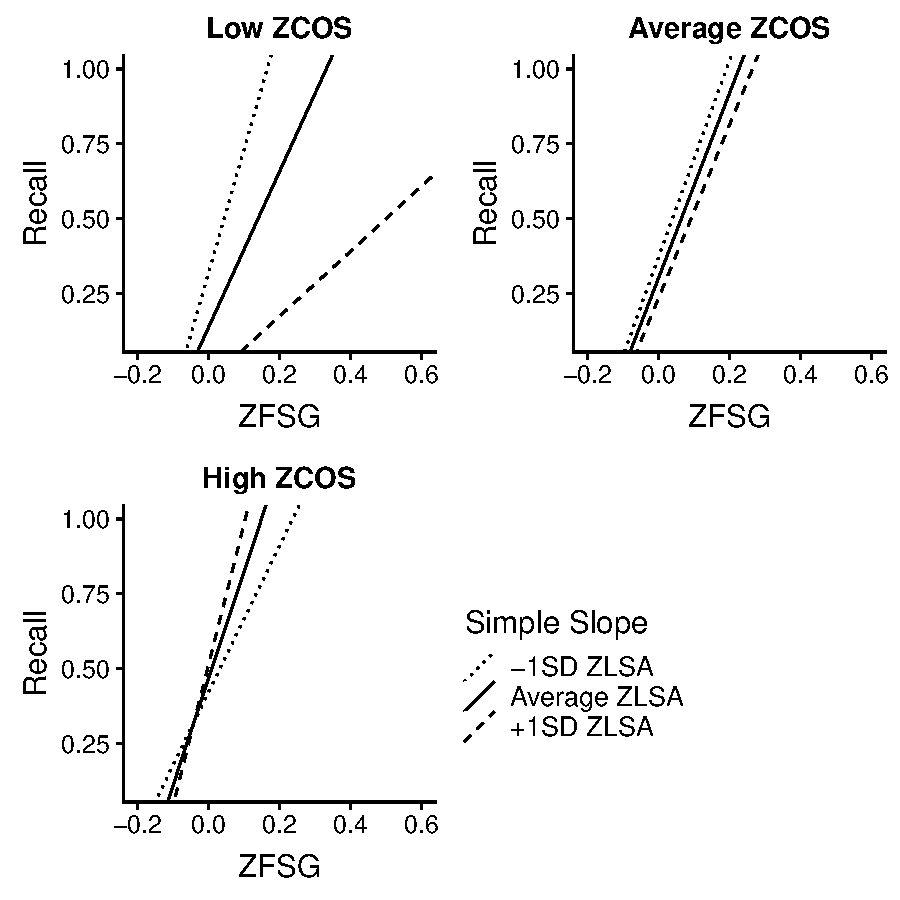
\includegraphics{max_buch_JOL_files/figure-latex/hyp3graph-1.pdf}
\caption{\label{fig:hyp3graph}Simple slopes graph displaying the slope of
FSG when predicting recall at low, average, and high LSA split by low,
average, and high COS. All variables were mean centered.}
\end{figure}

Given the results of Hypothesis 2, we then sought to extend the analysis
to participant recall scores. A multilevel logistic regression was used
with the \emph{lme4} package and \emph{glmer()} function (Pinheiro et
al., 2017), testing the interaction between FSG, COS, and LSA when
predicting participant recall. As with the previous hypothesis, we
controlled for type of judgement and, additionally, covaried judgment
ratings. Participants were used as a random intercept factor. Judged
values were a significant predictor of recall, (\(\beta\) = 0.686,
\emph{p} \textless{} .001) where increases in judged strength predicted
increases in recall. A significant three-way interaction was detected
between FSG, COS, and LSA (\(\beta\) = 24.572, \emph{p} \textless{}
.001). See Table \ref{tab:hyp3-table} for main effects, two-way, and
three-way interaction values.

The moderation process from Hypothesis 2 was then repeated, with simple
slopes first calculated at low, average, and high levels of COS. This
set of analyses resulted in significant two-way interactions between LSA
and FSG at low COS (\(\beta\) = -7.845, \emph{p} \textless{} .001) and
high COS (\(\beta\) = 5.811, \emph{p} = .009). No significant two-way
interaction was found at average COS (\(\beta\) = -1.017, \emph{p} =
.493). Following the design of hypothesis two, simple slopes were then
calculated for low, average, and high levels of LSA at the low and high
levels of COS, allowing us to assess how FSG effects recall at varying
levels of both COS and LSA. When both COS and LSA were low, FSG was a
significant predictor of recall (\(\beta\) = 4.116, \emph{p} \textless{}
.001). At low COS and average LSA, FSG decreased from both low levels,
but was still a significant predictor (\(\beta\) = 2.601, \emph{p}
\textless{} .001), and finally, low COS and high LSA, FSG was the
weakest predictor of the three (\(\beta\) = 1.086, \emph{p} = .030). As
with Hypothesis 2, LSA and FSG counterbalanced one another, wherein the
increasing levels of thematics led to a decrease in the importance of
association in predicting recall. At high COS and low LSA, FSG was a
significant predictor (\(\beta\) = 2.447, \emph{p} = .003). When COS was
high and LSA was average, FSG increased as a predictor and remained
significant (\(\beta\) = 3.569, \emph{p} \textless{} .001). This finding
repeated when both COS and LSA were high, with FSG increasing as a
predictor of recall (\(\beta\) = 4.692, \emph{p} \textless{} .001).
Therefore, at high levels of COS, LSA and FSG are complementary
predictors of recall, increasing together and extending the findings of
Hypothesis 2 to participant recall. Figure \ref{fig:hyp3graph} displays
the three-way interaction. The top left figure indicates the
counterbalancing effect of recall of LSA and FSG, while the top right
figure shows no differences in simple slopes for average levels of
cosine. The bottom left figure indicates the complementary effects where
LSA and FSG increase together as predictors of recall at high COS
levels.

\subsection{Hypothesis 4}\label{hypothesis-4}

\begin{table}[tbp]
\begin{center}
\begin{threeparttable}
\caption{\label{tab:hyp4-table}MLM Statistics for Hypothesis 4}
\begin{tabular}{lcccc}
\toprule
Variable & \multicolumn{1}{c}{$b$} & \multicolumn{1}{c}{$SE$} & \multicolumn{1}{c}{$z$} & \multicolumn{1}{c}{$p$}\\
\midrule
(Intercept) & -0.432 & 0.439 & -0.983 & .326\\
ACOS & 0.314 & 0.550 & 0.572 & .568\\
ALSA & 0.501 & 0.463 & 1.081 & .279\\
AFSG & 0.898 & 0.337 & 2.667 & .008\\
AIntercept & 1.514 & 0.604 & 2.507 & .012\\
(Intercept) & -0.827 & 0.463 & -1.787 & .074\\
SCOS & 2.039 & 0.518 & 3.939 & < .001\\
SLSA & 1.061 & 0.455 & 2.335 & .020\\
SFSG & 0.381 & 0.289 & 1.319 & .187\\
SIntercept & 2.292 & 0.681 & 3.363 & < .001\\
(Intercept) & 0.060 & 0.599 & 0.101 & .920\\
TCOS & 0.792 & 0.566 & 1.401 & .161\\
TLSA & 0.896 & 0.529 & 1.694 & .090\\
TFSG & -0.394 & 0.441 & -0.894 & .371\\
TIntercept & 1.028 & 0.756 & 1.360 & .174\\
\bottomrule
\addlinespace
\end{tabular}
\begin{tablenotes}[para]
\textit{Note.} Each judgment-database bias and sensitivity predicting recall for corresponding judgment block. A: Associative, S: Semantic, T: Thematic.
\end{tablenotes}
\end{threeparttable}
\end{center}
\end{table}

In our fourth and final hypothesis, we investigated whether the judgment
slopes and intercepts obtained in Hypothesis 1 would be predictive of
recall ability. Whereas Hypothesis 3 indicated that word relatedness was
directly related to recall performance, this hypothesis instead looked
at whether or not participants' sensitivity and bias to word relatedness
could be used a predictor of recall (Maki, 2007b). This analysis was
conducted with a multilevel logistic regression, as described in
Hypothesis 3 where each database slope and intercept was used as
predictors of recall using participant as a random intercept factor.
These analyses were separated by judgment type, so that each set of
judgment slopes and intercepts were used to predict recall. The
separation controlled for the number of variables in the equation, as
all slopes and intercepts would have resulted in overfitting. These
values were obtained from Hypothesis 1 where each participant's
individual slopes and intercepts were calculated for associative,
semantic, and thematic judgment conditions. Table \ref{tab:hyp1-table1}
shows average slopes and intercepts for recall for each of the three
types of memory, and Table \ref{tab:hyp4-table} portrays the regression
coefficients and statistics. In the associative condition, FSG slope
significantly predicted recall (\emph{b} = 0.898, \emph{p} = .008),
while COS slope (\emph{b} = 0.314, \emph{p} = .568) and LSA slope
(\emph{b} = 0.501, \emph{p} = .279) were non-significant. In the
semantic condition, COS slope (\emph{b} = 2.039, \emph{p} \textless{}
.001) and LSA slope (\emph{b} = 1.061, \emph{p} = .020) were both found
to be significant predictors of recall. FSG slope was non-significant in
this condition (\emph{b} = 0.381, \emph{p} = .187). Finally, no
predictors were significant in the thematic condition, though LSA slope
was found to be the strongest (\emph{b} = 0.896, \emph{p} = .090).

\section{Discussion}\label{discussion}

This study investigated the relationship between associative, semantic,
and thematic word relations and their effect on participant judgments
and recall performance through the testing of four hypotheses. In our
first hypothesis, bias and sensitivity findings first proposed by Maki
(2007a) were successfully replicated in the associative condition, with
slope and intercept values falling within the expected range. While
these findings were not fully replicated when extending the analysis to
include semantic and thematic judgments (as slopes in these conditions
did not fall within the appropriate range), participants still displayed
high intercepts and shallow slopes, suggesting overconfidence in
judgment making and an insensitivity to changes in strength between
pairs. Additionally, when looking at the frequency that each predictor
was the strongest in making these judgments, FSG was the best predictor
for both the associative and semantic conditions, while LSA was the best
predictor in the thematic condition. In each of the three conditions,
COS was the weakest predictor, even when participants were asked to make
semantic judgments. This finding suggests that associative relationships
seem to take precedence over semantic relationships when judging pair
relatedness, regardless of what type of judgment is elicited.
Additionally, this finding may be taken as further evidence of a
separation between associative information and semantic information, in
which associative information is always processed, while semantic
information may be suppressed due to task demands (Buchanan, 2010;
Hutchison \& Bosco, 2007).

Our second hypothesis examined the three-way interaction between FSG,
COS, and LSA when predicting participant judgments. At low semantic
overlap, a seesaw effect was found in which increases in thematic
strength led to decreases in associative predictiveness. This finding
was then replicated in hypothesis 3 when extending the analysis to
predict recall. By limiting the semantic relationships between pairs, an
increased importance is placed on the role of associations and thematics
when making judgments or retrieving pairs. In such cases, increasing the
amount of thematic overlap between pairs results in thematic
relationships taking precedent over associative relationships. However,
when semantic overlap was high, a complementary relationship was found
in which increases in thematic strength in turn led to increases in the
strength of FSG as a predictor. This result suggests that at high
semantic overlap, associations and thematic relations build upon one
another. Because thematics is tied to both semantic overlap and item
associations, the presence of strong thematic relationships between
pairs during conditions of high semantic overlap boosts the predictive
ability of associative word norms. Again, this complementary effect was
found when examining both recall and judgments.

Finally, our fourth hypothesis used the judgment slopes and intercepts
calculated in Hypothesis 1 to investigate if participants' bias and
sensitivity to word relatedness could be used to predict recall. For the
associative condition, the FSG slope significantly predicted recall. In
the semantic condition, recall was significantly predicted by both the
COS and LSA slopes. However, for the thematic condition, although the
LSA slope was the strongest, no predictors were significant. One
explanation for this finding is that thematic relationships between item
pairs act as a blend between associations and semantics. As such, LSA
faces increased competition from the associative and semantic database
norms when predicting recall in this manner.

Overall, our findings indicated the degree to which the processing of
associative, semantic, and thematic information impacts retrieval and
judgment making tasks and the interactive relationship that exists
between these three types of lexical information. While previous
research has shown that memory networks are divided into separate
systems which handle storage and processing for meaning and association,
the presence of these interactions suggests that connections exist
between these networks, linking them to one another. As such, we suggest
that these memory systems may form a three-tiered, interconnected
system. First, information enters the semantic memory network, which
processes features of concepts and provides a means of categorizing
items based on the similarity of their features. Next, the associative
network adds information for items based on contexts generated by
reading or speech. Finally, the thematic network pulls in information
from both the semantic and associative networks to create a mental
representation of both the item and its place world relative to other
concepts. This study did not explore the timing of information input
from each of these systems, but it may be similar to a dual-route model
of reading and naming, in that each runs in parallel contributing the
judgment and recall process (Coltheart, Curtis, Atkins, \& Haller,
1993).

Viewing this model purely through the lens of semantic memory, it draws
comparison to dynamic attractor models (Hopfield, 1982; Jones et al.,
2015; McLeod et al., 2000). One of the defining features of dynamic
attractor models is that they allow for some type of bidirectionally or
feedback between connections in the network. In the study of semantic
memory, these models are useful for taking into account multiple
restraints such as links between semantics and the orthography of the
concept in question. Our hypothesis extends this notion as a means of
framing how these three memory systems are connected. The underlying
meaning of a concept is linked with both information pertaining to its
co-occurrences in everyday language and information relating to the
general contexts in which it typically appears.

How then does this hypothesis lend itself towards the broader context of
psycholinguistic research? One application of this hypothesis may be
models of word recognition. One popular model is Seidenberg and
Mcclelland (1989) \enquote{triangle model}, and several variations of
this model have been proposed and tested (see Harley, 2008 for a
review). This model recognizes speech and reading based upon the
orthography, phonology, and meaning of words. Each of these three word
properties are linked to in such a way that orthography is linked to
phonology, phonology is linked with meaning, and meaning is linked to
orthography (forming a triangle). The pathways between word properties
are bidirectional, allowing for feedback between connections. Whereas
the original version of this model focused almost exclusively on the
link between orthography and phonology, Harm and Seidenberg (2004)
developed a version which included a focus on semantics, with word
meaning being based on input from the orthography and phonology
components of the model. Future studies in this area may wish to
incorporate thematic and associative knowledge as elements of meaning,
as thematic and associative information is interconnected with the
semantic network. Ultimately, further studies will be needed to explore
the interconnections between the semantic, thematic, and associative
networks.

\newpage

\section{References}\label{references}

\setlength{\parindent}{-0.5in} \setlength{\leftskip}{0.5in}

\hypertarget{refs}{}
\hypertarget{ref-R-papaja}{}
Aust, F., \& Barth, M. (2017). \emph{papaja: Create APA manuscripts with
R Markdown}. Retrieved from \url{https://github.com/crsh/papaja}

\hypertarget{ref-Bates2015}{}
Bates, D., Mächler, M., Bolker, B., \& Walker, S. (2015). Fitting linear
mixed-effects models using lme4. \emph{Journal of Statistical Software},
\emph{67}(1), 1--48.
doi:\href{https://doi.org/10.18637/jss.v067.i01}{10.18637/jss.v067.i01}

\hypertarget{ref-Buchanan2010}{}
Buchanan, E. M. (2010). Access into memory: Differences in judgments and
priming for semantic and associative memory. \emph{Journal of Scientific
Psychology}, \emph{March}, 1--8.

\hypertarget{ref-Buchanan2013}{}
Buchanan, E. M., Holmes, J. L., Teasley, M. L., \& Hutchison, K. A.
(2013). English semantic word-pair norms and a searchable Web portal for
experimental stimulus creation. \emph{Behavior Research Methods},
\emph{45}(3), 746--757.
doi:\href{https://doi.org/10.3758/s13428-012-0284-z}{10.3758/s13428-012-0284-z}

\hypertarget{ref-Buhrmester2011}{}
Buhrmester, M., Kwang, T., \& Gosling, S. D. (2011). Amazon's Mechanical
Turk. \emph{Perspectives on Psychological Science}, \emph{6}(1), 3--5.
doi:\href{https://doi.org/10.1177/1745691610393980}{10.1177/1745691610393980}

\hypertarget{ref-Chow2014}{}
Chow, B. W.-Y. (2014). The differential roles of paired associate
learning in Chinese and English word reading abilities in bilingual
children. \emph{Reading and Writing}, \emph{27}(9), 1657--1672.
doi:\href{https://doi.org/10.1007/s11145-014-9514-3}{10.1007/s11145-014-9514-3}

\hypertarget{ref-Coltheart1993}{}
Coltheart, M., Curtis, B., Atkins, P., \& Haller, M. (1993). Models of
reading aloud: Dual-route and parallel-distributed-processing
approaches. \emph{Psychological Review}, \emph{100}(4), 589--608.
doi:\href{https://doi.org/10.1037//0033-295X.100.4.589}{10.1037//0033-295X.100.4.589}

\hypertarget{ref-Gelman2006}{}
Gelman, A. (2006). Multilevel (hierarchical) modeling: What it can and
cannot do. \emph{Technometrics}, \emph{48}(3), 432--435.
doi:\href{https://doi.org/10.1198/004017005000000661}{10.1198/004017005000000661}

\hypertarget{ref-Green2016}{}
Green, P., \& MacLeod, C. J. (2016). SIMR: an R package for power
analysis of generalized linear mixed models by simulation. \emph{Methods
in Ecology and Evolution}, \emph{7}(4), 493--498.
doi:\href{https://doi.org/10.1111/2041-210X.12504}{10.1111/2041-210X.12504}

\hypertarget{ref-Harley2008}{}
Harley, T. (2008). \emph{The psychology of language: From data to
theory} (3rd ed.). New York: Psychology Press.

\hypertarget{ref-Harm2004}{}
Harm, M. W., \& Seidenberg, M. S. (2004). Computing the meanings of
words in reading: Cooperative division of labor between visual and
phonological processes. \emph{Psychological Review}, \emph{111}(3),
662--720.
doi:\href{https://doi.org/10.1037/0033-295X.111.3.662}{10.1037/0033-295X.111.3.662}

\hypertarget{ref-Hertzog2002}{}
Hertzog, C., Kidder, D. P., Powell-Moman, A., \& Dunlosky, J. (2002).
Aging and monitoring associative learning: Is monitoring accuracy spared
or impaired? \emph{Psychology and Aging}, \emph{17}(2), 209--225.
doi:\href{https://doi.org/10.1037/0882-7974.17.2.209}{10.1037/0882-7974.17.2.209}

\hypertarget{ref-Hopfield1982}{}
Hopfield, J. J. (1982). Neural networks and physical systems with
emergent collective computational abilities. \emph{Proceedings of the
National Academy of Sciences}, \emph{79}(8), 2554--2558.
doi:\href{https://doi.org/10.1073/pnas.79.8.2554}{10.1073/pnas.79.8.2554}

\hypertarget{ref-Hutchison2003}{}
Hutchison, K. A. (2003). Is semantic priming due to association strength
or feature overlap? A microanalytic review. \emph{Psychonomic Bulletin
\& Review}, \emph{10}(4), 785--813.
doi:\href{https://doi.org/10.3758/BF03196544}{10.3758/BF03196544}

\hypertarget{ref-Hutchison2007}{}
Hutchison, K. A., \& Bosco, F. A. (2007). Congruency effects in the
letter search task: semantic activation in the absence of priming.
\emph{Memory \& Cognition}, \emph{35}(3), 514--525.
doi:\href{https://doi.org/10.3758/BF03193291}{10.3758/BF03193291}

\hypertarget{ref-Jiang1997}{}
Jiang, J. J., \& Conrath, D. W. (1997). Semantic similarity based on
corpus statistics and lexical taxonomy. \emph{Proceedings of
International Conference Research on Computational Linguistics}, 19--33.
Retrieved from \url{http://arxiv.org/abs/cmp-lg/9709008}

\hypertarget{ref-Jones2012}{}
Jones, L. L., \& Golonka, S. (2012). Different influences on lexical
priming for integrative, thematic, and taxonomic relations.
\emph{Frontiers in Human Neuroscience}, \emph{6}, 1--17.
doi:\href{https://doi.org/10.3389/fnhum.2012.00205}{10.3389/fnhum.2012.00205}

\hypertarget{ref-Jones2015}{}
Jones, M. N., Willits, J., \& Dennis, S. (2015). Models of semantic
memory. In A. T. Townsend \& Jerome R. Busemeyer (Eds.), \emph{Oxford
handbook of mathematical and computational psychology} (pp. 232--254).
Oxford University Press.
doi:\href{https://doi.org/10.1093/oxfordhb/9780199957996.013.11}{10.1093/oxfordhb/9780199957996.013.11}

\hypertarget{ref-Jouravlev2016}{}
Jouravlev, O., \& McRae, K. (2016). Thematic relatedness production
norms for 100 object concepts. \emph{Behavior Research Methods},
\emph{48}(4), 1349--1357.
doi:\href{https://doi.org/10.3758/s13428-015-0679-8}{10.3758/s13428-015-0679-8}

\hypertarget{ref-Koriat2005}{}
Koriat, A., \& Bjork, R. A. (2005). Illusions of competence in
monitoring one's knowledge during study. \emph{Journal of Experimental
Psychology: Learning, Memory, and Cognition}, \emph{31}(2), 187--194.
doi:\href{https://doi.org/10.1037/0278-7393.31.2.187}{10.1037/0278-7393.31.2.187}

\hypertarget{ref-Landauer1997}{}
Landauer, T. K., \& Dumais, S. T. (1997). A solution to Plato's problem:
The latent semantic analysis theory of acquisition, induction, and
representation of knowledge. \emph{Psychological Review}, \emph{104}(2),
211--240.
doi:\href{https://doi.org/10.1037//0033-295X.104.2.211}{10.1037//0033-295X.104.2.211}

\hypertarget{ref-Landauer1998}{}
Landauer, T. K., Foltz, P. W., \& Laham, D. (1998). An introduction to
latent semantic analysis. \emph{Discourse Processes}, \emph{25}(2),
259--284.
doi:\href{https://doi.org/10.1080/01638539809545028}{10.1080/01638539809545028}

\hypertarget{ref-Lucas2000}{}
Lucas, M. (2000). Semantic priming without association: a meta-analytic
review. \emph{Psychonomic Bulletin \& Review}, \emph{7}(4), 618--630.
doi:\href{https://doi.org/10.3758/BF03212999}{10.3758/BF03212999}

\hypertarget{ref-Lund1996}{}
Lund, K., \& Burgess, C. (1996). Producing high-dimensional semantic
spaces from lexical co-occurrence. \emph{Behavior Research Methods,
Instruments, \& Computers}, \emph{28}(2), 203--208.
doi:\href{https://doi.org/10.3758/BF03204766}{10.3758/BF03204766}

\hypertarget{ref-Maki2007a}{}
Maki, W. S. (2007a). Judgments of associative memory. \emph{Cognitive
Psychology}, \emph{54}(4), 319--353.
doi:\href{https://doi.org/10.1016/j.cogpsych.2006.08.002}{10.1016/j.cogpsych.2006.08.002}

\hypertarget{ref-Maki2007}{}
Maki, W. S. (2007b). Separating bias and sensitivity in judgments of
associative memory. \emph{Journal of Experimental Psychology: Learning,
Memory, and Cognition}, \emph{33}(1), 231--237.
doi:\href{https://doi.org/10.1037/0278-7393.33.1.231}{10.1037/0278-7393.33.1.231}

\hypertarget{ref-Maki2008}{}
Maki, W. S., \& Buchanan, E. M. (2008). Latent structure in measures of
associative, semantic, and thematic knowledge. \emph{Psychonomic
Bulletin \& Review}, \emph{15}(3), 598--603.
doi:\href{https://doi.org/10.3758/PBR.15.3.598}{10.3758/PBR.15.3.598}

\hypertarget{ref-Maki2004}{}
Maki, W. S., McKinley, L. N., \& Thompson, A. G. (2004). Semantic
distance norms computed from an electronic dictionary (WordNet).
\emph{Behavior Research Methods, Instruments, \& Computers},
\emph{36}(3), 421--431.
doi:\href{https://doi.org/10.3758/BF03195590}{10.3758/BF03195590}

\hypertarget{ref-McLeod2000}{}
McLeod, P., Shallice, T., \& Plaut, D. C. (2000). Attractor dynamics in
word recognition: converging evidence from errors by normal subjects,
dyslexic patients and a connectionist model. \emph{Cognition},
\emph{74}(1), 91--114.
doi:\href{https://doi.org/10.1016/S0010-0277(99)00067-0}{10.1016/S0010-0277(99)00067-0}

\hypertarget{ref-McRae2005}{}
McRae, K., Cree, G. S., Seidenberg, M. S., \& McNorgan, C. (2005).
Semantic feature production norms for a large set of living and
nonliving things. \emph{Behavior Research Methods}, \emph{37}(4),
547--559.
doi:\href{https://doi.org/10.3758/BRM.40.1.183}{10.3758/BRM.40.1.183}

\hypertarget{ref-Meyer1971}{}
Meyer, D. E., \& Schvaneveldt, R. W. (1971). Facilitation in recognizing
pairs of words: Evidence of a dependence between retrieval operations.
\emph{Journal of Experimental Psychology}, \emph{90}(2), 227--234.
doi:\href{https://doi.org/10.1037/h0031564}{10.1037/h0031564}

\hypertarget{ref-Meyer1975}{}
Meyer, D. E., Schvaneveldt, R. W., \& Ruddy, M. G. (1975). Loci of
contextual effects on visual word-recognition. In P. M. A. Rabbitt
(Ed.), \emph{Attention and performance v}. London, UK: Academic Press.

\hypertarget{ref-Miller1995}{}
Miller, G. A. (1995). WordNet: a lexical database for English.
\emph{Communications of the ACM}, \emph{38}(11), 39--41.
doi:\href{https://doi.org/10.1145/219717.219748}{10.1145/219717.219748}

\hypertarget{ref-Nelson2000}{}
Nelson, D. L., McEvoy, C. L., \& Dennis, S. (2000). What is free
association and what does it measure? \emph{Memory \& Cognition},
\emph{28}(6), 887--899.
doi:\href{https://doi.org/10.3758/BF03209337}{10.3758/BF03209337}

\hypertarget{ref-Nelson2004}{}
Nelson, D. L., McEvoy, C. L., \& Schreiber, T. A. (2004). The University
of South Florida free association, rhyme, and word fragment norms.
\emph{Behavior Research Methods, Instruments, \& Computers},
\emph{36}(3), 402--407.
doi:\href{https://doi.org/10.3758/BF03195588}{10.3758/BF03195588}

\hypertarget{ref-Paivio1969}{}
Paivio, A. (1969). Mental imagery in associative learning and memory.
\emph{Psychological Review}, \emph{76}(3), 241--263.
doi:\href{https://doi.org/10.1037/h0027272}{10.1037/h0027272}

\hypertarget{ref-Pinheiro2017}{}
Pinheiro, J., Bates, D., Debroy, S., Sarkar, D., \& R Core Team. (2017).
nlme: Linear and Nonlinear Mixed Effects Models. Retrieved from
\url{https://cran.r-project.org/package=nlme}

\hypertarget{ref-Plaut1996}{}
Plaut, D. C., McClelland, J. L., Seidenberg, M. S., \& Patterson, K.
(1996). Understanding normal and impaired word reading: Computational
principles in quasi-regular domains. \emph{Psychological Review},
\emph{103}(1), 56--115.
doi:\href{https://doi.org/10.1037//0033-295X.103.1.56}{10.1037//0033-295X.103.1.56}

\hypertarget{ref-Richardson1998}{}
Richardson, J. T. E. (1998). The availability and effectiveness of
reported mediators in associative learning: A historical review and an
experimental investigation. \emph{Psychonomic Bulletin \& Review},
\emph{5}(4), 597--614.
doi:\href{https://doi.org/10.3758/BF03208837}{10.3758/BF03208837}

\hypertarget{ref-Riordan2011}{}
Riordan, B., \& Jones, M. N. (2011). Redundancy in perceptual and
linguistic experience: Comparing feature-based and distributional models
of semantic representation. \emph{Topics in Cognitive Science},
\emph{3}(2), 303--345.
doi:\href{https://doi.org/10.1111/j.1756-8765.2010.01111.x}{10.1111/j.1756-8765.2010.01111.x}

\hypertarget{ref-Rogers2006}{}
Rogers, T. T., \& McClelland, J. L. (2006). \emph{Semantic cognition}.
Cambridge, MA: MIT Press.

\hypertarget{ref-Rumelhart1986}{}
Rumelhart, D. E., McClelland, J. L., \& Group, P. R. (1986).
\emph{Parallel distributed processing: Explorations in the
microstructure of cognition. Volume 1}. Cambridge, MA: MIT Press.

\hypertarget{ref-Schwartz2013}{}
Schwartz, B. L., \& Brothers, B. R. (2013). Survival processing does not
improve paired-associate learning. In B. L. Schwartz, M. L. Howe, M. P.
Toglia, \& H. Otgaar (Eds.), \emph{What is adaptive about adaptive
memory?} (pp. 159--171). Oxford University Press.
doi:\href{https://doi.org/10.1093/acprof:oso/9780199928057.003.0009}{10.1093/acprof:oso/9780199928057.003.0009}

\hypertarget{ref-Seidenberg1989}{}
Seidenberg, M. S., \& Mcclelland, J. L. (1989). A distributed,
developmental model of word recognition and naming. \emph{Psychological
Review}, \emph{96}, 523--568.

\hypertarget{ref-Smythe1968}{}
Smythe, P. C., \& Paivio, A. (1968). A comparison of the effectiveness
of word imagery and meaningfulness in paired-associate learning of
nouns. \emph{Psychonomic Science}, \emph{10}(2), 49--50.
doi:\href{https://doi.org/10.3758/BF03331401}{10.3758/BF03331401}

\hypertarget{ref-Tabachnick2007}{}
Tabachnick, B. G., \& Fidell, L. S. (2007). \emph{Using Multivariate
Statistics} (5th ed.). New York, NY: Allyn \& Bacon.

\hypertarget{ref-Valentine2013}{}
Valentine, K. D., \& Buchanan, E. M. (2013). JAM-boree: An application
of observation oriented modelling to judgements of associative memory.
\emph{Journal of Cognitive Psychology}, \emph{25}(4), 400--422.
doi:\href{https://doi.org/10.1080/20445911.2013.775120}{10.1080/20445911.2013.775120}

\hypertarget{ref-Vinson2008}{}
Vinson, D. P., \& Vigliocco, G. (2008). Semantic feature production
norms for a large set of objects and events. \emph{Behavior Research
Methods}, \emph{40}(1), 183--190.
doi:\href{https://doi.org/10.3758/BRM.40.1.183}{10.3758/BRM.40.1.183}

\hypertarget{ref-Wickham2007}{}
Wickham, H. (2007). Reshaping data with the reshape package.
\emph{Journal of Statistical Software}, \emph{21}(12).
doi:\href{https://doi.org/10.18637/jss.v021.i12}{10.18637/jss.v021.i12}






\end{document}
